\documentclass[11pt,a4paper,oneside]{book}
\usepackage[a4paper,margin=22mm]{geometry}
\usepackage[T1]{fontenc}
\usepackage{newtxtext,newtxmath}
\usepackage{microtype}
\usepackage{booktabs}
\usepackage{graphicx}
\usepackage{float}
\usepackage{xcolor}
\usepackage{enumitem}
\usepackage[most]{tcolorbox}
\usepackage[hidelinks]{hyperref}
\setlist{itemsep=1pt,topsep=3pt}
\setlist[enumerate]{label=\arabic*.}
\graphicspath{{fig/}}
\newcommand{\MCargoMax}{20\,000}
\newcommand{\MClimbLeast}{1\,370}
\newcommand{\MClimbLeastKt}{250}
\newcommand{\MClimbWeight}{47\,500}
\newcommand{\MFuelGal}{1\,448}
\newcommand{\MFuelLb}{9\,860}
\newcommand{\MMmo}{0.48}
\newcommand{\MNacMax}{97.5}
\newcommand{\MNacMin}{0}
\newcommand{\MNacRate}{8}
\newcommand{\MNrApln}{84}
\newcommand{\MNrHelo}{104}
\newcommand{\MOeiHoverPower}{6\,944}
\newcommand{\MOeiLo}{80}
\newcommand{\MPirp}{5\,904}
\newcommand{\MPitchTwoFifty}{3}
\newcommand{\MPitchTwoHundred}{6}
\newcommand{\MPitchTwoSeventy}{2}
\newcommand{\MPmcp}{4\,982}
\newcommand{\MPmrp}{6\,150}
\newcommand{\MPoneThousand}{5\,950}
\newcommand{\MPxmsn}{9\,130}
\newcommand{\MPxmsnApln}{7\,669}
\newcommand{\MRotorDia}{38}
\newcommand{\MSpan}{45.8}
\newcommand{\MTfHorizon}{45}
\newcommand{\MTfRise}{950}
\newcommand{\MTroops}{24}
\newcommand{\MVmo}{280}
\newcommand{\MVmoHundred}{220}
\newcommand{\MVrsHiKt}{60}
\newcommand{\MVrsHiSink}{1\,600}
\newcommand{\MVrsLoKt}{30}
\newcommand{\MVrsLoSink}{800}
\newcommand{\MWEmpty}{33\,140}
\newcommand{\MWRef}{47\,500}
\newcommand{\MWStart}{38\,730}

\newcommand{\Tab}[1]{\input{tab/tab_#1.tex}}
\newcommand{\key}[1]{\texttt{#1}}
% a display's picture (disp/<name>.png, capture.py) with its numbered callouts beside it (figures.py)
\newcommand{\DispFig}[3]{\begin{figure}[H]\centering
  \begin{minipage}[c]{#2}\includegraphics[width=\linewidth]{disp_#1.pdf}\end{minipage}\hfill
  \begin{minipage}[c]{\dimexpr\textwidth-#2-6mm\relax}\small\input{tab/callouts_#1.tex}\end{minipage}
  \caption{#3}\label{fig:#1}\end{figure}}
\newcommand{\DispPair}[5]{\begin{figure}[H]\centering
  \begin{minipage}[t]{0.48\textwidth}\centering\includegraphics[width=\linewidth]{disp_#1.pdf}\par\small(a) #2\end{minipage}\hfill
  \begin{minipage}[t]{0.48\textwidth}\centering\includegraphics[width=\linewidth]{disp_#3.pdf}\par\small(b) #4\end{minipage}
  \caption{#5}\label{fig:#1}\end{figure}}
\newcommand{\ann}[1]{\textsf{#1}}
% WARNING, CAUTION and NOTE, as flight manuals set them
\newtcolorbox{warning}{enhanced,colback=white,colframe=black,boxrule=1.2pt,arc=0pt,left=6pt,right=6pt,top=3pt,bottom=4pt,
  title={\centering\bfseries WARNING},coltitle=black,colbacktitle=white,titlerule=0pt,fonttitle=\normalsize}
\newtcolorbox{caution}{enhanced,colback=white,colframe=black,boxrule=0.6pt,arc=0pt,left=6pt,right=6pt,top=3pt,bottom=4pt,
  title={\centering\bfseries CAUTION},coltitle=black,colbacktitle=white,titlerule=0pt,fonttitle=\normalsize}
\newtcolorbox{note}{enhanced,colback=white,colframe=white,boxrule=0pt,left=6pt,right=6pt,top=2pt,bottom=2pt,
  title={\centering\bfseries Note},coltitle=black,colbacktitle=white,titlerule=0pt,fonttitle=\normalsize}

\begin{document}
\frontmatter
\begin{titlepage}
\centering
\vspace*{50mm}
{\Huge\bfseries MV-22B Osprey\par}
\vspace{6mm}
{\LARGE Flight Manual\par}
\vspace{4mm}
{\large for the FlightGear MV-22B with its JSBSim flight model\par}
\vspace{30mm}
\begin{minipage}{0.75\textwidth}\small
This manual describes the aircraft as simulated: its flight model, cockpit, displays and automatic flight control
system. Much of it has no counterpart in the real aircraft, whose manual is not public, and none of it is the real
aircraft's manual or procedures. It is generated with the aircraft: its numbers, tables and charts come from the
aircraft's own data, so they follow it as it changes.
\end{minipage}
\vfill
{\small Generated from the aircraft's sources (\texttt{manual/} in its repository).\par}
\end{titlepage}

\chapter*{How to use this manual}
\addcontentsline{toc}{chapter}{How to use this manual}
The manual is in parts, as a military flight manual is: the aircraft and its systems (Part~I), its limitations (Part~II),
normal procedures (Part~III), flight characteristics (Part~IV), emergency procedures (Part~V) and performance data
(Part~VI). Keys are given as \key{m} or \key{Ctrl-T}; words the displays show, as \ann{HVR CPLD HOLD}.

\paragraph{Warnings, cautions and notes.} Three kinds of notice stand apart from the text, by how much they matter:
\begin{warning}
An operating procedure or technique that, not followed, may lose the aircraft.
\end{warning}
\begin{caution}
An operating procedure or technique that, not followed, may damage the aircraft or end the flight's purpose.
\end{caution}
\begin{note}
An operating procedure, technique or fact worth emphasising.
\end{note}

\paragraph{Wording.} \emph{Shall} is mandatory; \emph{should} is recommended; \emph{may} and \emph{need not} are optional;
\emph{will} states what happens, not a requirement.

\paragraph{Its numbers.} Weights are pounds, speeds knots (KCAS, calibrated, unless stated), heights feet, power shaft
horsepower. Performance is the flight model's: the comparisons that support it are in the model's report.

\tableofcontents

\mainmatter
% =====================================================================================================================
\part{The aircraft}
\chapter{General description}
\section{The aircraft}
The MV-22B is a tiltrotor: two proprotors, \MRotorDia{}\,ft across, at the tips of a wing, on nacelles that tilt from
vertical (90$^\circ$, helicopter mode) to horizontal (0$^\circ$, airplane mode) and \MNacMax{}$-$90 = 7.5$^\circ$ aft
of vertical. In helicopter mode the rotors lift the aircraft and it hovers and manoeuvres as a helicopter does; in
airplane mode the wing lifts it and the rotors are propellers. Between them it \emph{converts}, the nacelles moving
at up to \MNacRate$^\circ$/s within a corridor of nacelle angle against airspeed (Part~II).

Two engines drive the rotors through gearboxes and an interconnect shaft: either engine turns both rotors. The flight
controls mix the pilot's controls into each mode's: the rotors' collective and cyclic in helicopter mode, the
elevator, flaperons and rudders in airplane mode, both through the conversion. A fly-by-wire augmentation holds
attitude in every mode, and an automatic flight control system (AFCS) flies the aircraft when coupled, down to a
hover and a landing.

\section{Weights}
\begin{center}\small
\begin{tabular}{@{}lr@{}}
\toprule
Empty & \MWEmpty \\
At the start: three crew, tanks half full, no cargo & \MWStart \\
Reference loading (maximum vertical take-off weight of the 1986 design) & \MWRef \\
Fuel, full (\MFuelGal\,US gal) & \MFuelLb \\
Troops and cargo in the cabin, up to & \MCargoMax \\
\bottomrule
\end{tabular}
\end{center}
Fuel and cargo are set from Equipment $\rightarrow$ Fuel and Payload; the Troops and cargo slider places the load in
the cabin. \MTroops{} equipped troops weigh about 5800\,lb.

% =====================================================================================================================
\chapter{Systems}
\section{Engines and drive}
Each engine is rated at \MPmrp\,shp (maximum rated power; intermediate \MPirp, maximum continuous \MPmcp), falling
with altitude and temperature. The thrust control lever sets both engines' power demand from flight idle to the
rating. The drive limits the torque: \MPxmsn\,hp at 100\,\% rotor speed, \MPxmsnApln\,hp at 84\,\%, shared between the
running engines, so that near sea level the drive, not the engines, limits the power. A governor holds the rotor
speed ($N_R$) with the rotors' collective: \MNrHelo\,\% in helicopter mode and through the conversion, \MNrApln\,\% in
airplane mode with the nacelles at 0$^\circ$. A topping governor takes power off above 2\,\% of overspeed.

The ENG format shows each engine's torque, gas generator speed and fuel flow, the rotor speed and the drive's
torque limit. Cautions: \ann{TORQUE} above 100\,\% torque, \ann{NR} with the rotor speed 3\,\% off its reference,
\ann{ENG 1 OUT} or \ann{ENG 2 OUT} with one engine stopped.

\section{Fuel}
Five tanks, drawn in the transfer sequence's order: the right aft sponson first, then the forward sponsons, the feed
tanks last.
\begin{center}\small\Tab{tanks}\end{center}
The FUEL format shows the tanks, the flow and the endurance; the NAV format the endurance and range. \ann{FUEL LOW}
shows below 1000\,lb.

\section{Flight controls}
\paragraph{Thrust control lever (TCL).} The throttle axis, or \key{Page Up}/\key{Page Down}. Up is more collective in
helicopter mode and more power in airplane mode. At the start's weight a hover needs about two thirds of it, at the
reference loading nearly all.

\paragraph{Nacelles.} \key{m} tilts the nacelle command 10$^\circ$ forward, \key{M} 10$^\circ$ aft; the NACELLE
thumbwheel on either lever does the same (click it, or the mouse wheel over it). The nacelles follow the command at
the conversion rate. From 90$^\circ$ \key{M} tilts them to \MNacMax$^\circ$, 7.5$^\circ$ aft of vertical, to stop or
back up in the hover.

\paragraph{Conversion protection.} The command is held within the corridor (Part~II): below 35\,kt the nacelles go no
further forward than 75$^\circ$, and as the aircraft accelerates they follow the corridor's lower edge, so a command
fully forward converts as the speed allows. Slowing below the corridor for the present angle, the protection raises
them. \ann{CONV PROT} shows while it holds the command off the pilot's.

\paragraph{Stick and pedals.} The elevator and aileron axes and the rudder axis. The flight controls mix them into the
rotors' cyclic and differential collective in helicopter mode, phased with the nacelles, and into the elevator,
flaperons and rudders in every mode.

\paragraph{Flaperons.} Scheduled by the flight model: 67$^\circ$ in the hover (least download), 40$^\circ$ through the
conversion and in airplane mode below 120\,kt, retracted by 200\,kt. The flap lever on the console does nothing.

\section{Flight control augmentation}
The augmentation holds the aircraft's attitude in all modes. Its response type changes with speed:
\begin{itemize}
\item \emph{Below 50\,kt with the nacelles above 60$^\circ$}: attitude command, heading hold. Each 5\,\% of stick (one
arrow-key press) holds about 1$^\circ$ of pitch or 1.25$^\circ$ of bank; each 5\,\% of pedal turns the aircraft at
1.5$^\circ$/s (30$^\circ$/s at full travel), and the heading holds with the pedals centred.
\item \emph{Above it}: rate command, attitude hold. The stick commands a rate, and the aircraft holds the attitude it
is released at.
\end{itemize}
It switches at 55\,kt accelerating and 45\,kt slowing, so that a speed held near 50\,kt does not switch back and forth;
both share one reference, so the switch is free of transients. A trim schedule keeps the stick's centre trimmed
through the conversion: hands off, the aircraft holds its attitude through it.

\section{Landing gear, brakes and the wing}
\key{g}/\key{G} raise and lower the gear; \ann{GEAR DOWN} shows with the gear down above 150\,kt and 50\,ft. \key{B}
sets the parking brake. The rotor brake holds the stopped rotors (\ann{ROTOR BRAKE}); the start releases it. \key{N}
folds the blades and swings the wing along the fuselage, \key{n} unfolds it; the rotors shall be stopped.

\section{Doors, lights and others}
\key{d} crew door, \key{D} cargo doors, \key{e} steps, \key{l} landing light. The complete list of keys is in
Table~\ref{tab:keys}.

% =====================================================================================================================
\chapter{Cockpit and displays}
\section{Layout}
Four multifunction displays (MFD~1 to 4 from the left) across the instrument panel; the control display unit (CDU)
and its two keypads on the centre console with the standby engine and fuel display (SFD) above it; the electronic
standby flight instrument (ESFI); the flight control panel (the AFCS's keys and knobs) and the radio panels on the
glareshield; a thrust control lever beside each seat.

\section{Multifunction displays}
The keys along each display's top pick its format: FLT, NAV, ENG, FUEL. A format's own keys, down its right side, show
their labels for a few seconds after a key is pressed.

\paragraph{Flight (FLT).} One format for every regime (Figure~\ref{fig:flt_airplane}). At its centre the flight path marker, where the aircraft is
going, with its acceleration chevron; airspeed and altitude tapes with 10\,s trend vectors; the heading; a ground grid
in perspective. The limits are drawn where the eye already is: the conversion corridor's airspeeds for the present
nacelle angle on the airspeed tape, the high sink rate boundary for the airspeed on the vertical speed scale (its bar
turning amber, then red, as the descent nears it), and the margin to the first power limit as one bar, with the power
to hover in and out of ground effect marked. A small corridor diagram shows where the aircraft is in the conversion and
where it is going. The AFCS's mode line runs along its top (Section~\ref{sec:annunciation}).
\DispFig{flt_airplane}{0.55\textwidth}{The flight format in airplane mode, coupled at 230\,kt.}

Slowing below 30\,kt with the nacelles past 75$^\circ$ it turns to its \emph{hover format} (Figure~\ref{fig:flt_hover}): the flight path marker
gives way to the drift seen from above, a ball on a line from the centre at the ground velocity's opposite 3\,s ahead,
to fly the stick towards; the hover hold's point, a magenta box filled once it holds it; the radar height. Below
200\,ft the height tape gives way to a green bar under the readout that drains to its foot as the height goes, at the
rate the aircraft closes on the ground. Past 60$^\circ$ of bank or 25$^\circ$ of pitch the clutter goes and an arrow
shows the way to roll level. R7 (HVR MARK) marks the present position as a hover point.
\DispFig{flt_hover}{0.55\textwidth}{The flight format's hover format, the hover hold holding 150\,ft over the sea.}

\paragraph{Navigation (NAV).} A moving map, track up (R3: north up; Figure~\ref{fig:nav}). The terrain is coloured by its clearance below the
height the aircraft will have when it gets there (60\,s ahead at most; below 90\,kt in the helicopter's tighter bands);
where the scenery has no elevation yet it is dim magenta, and below 100\,ft above the ground it is measured from 100\,ft
up, so that flat ground around a hover stays quiet. On it: the route and its waypoints; the landing zone, the route's
last point, with its approach into the wind; the conversion planner's points, where to begin slowing down (DECEL) and
converting (CONV) to arrive in a hover; the path 30 and 60\,s ahead in the turn; an approach line; traffic; the fuel's
endurance and range. Below it the profile along the track: the terrain, the aircraft's path, the selected altitude.
R1/R2 change the range, R4 the terrain.
\DispFig{nav}{0.55\textwidth}{The navigation format with a route over the peninsula's ridge to a landing zone on the coast, at
120\,kt: the terrain beyond the coast not yet loaded by the scenery.}

\paragraph{Engines (ENG)} and \textbf{fuel (FUEL)}: the engines and drive, the tanks and the flow
(Figures~\ref{fig:eng} and~\ref{fig:fuel}).
\DispFig{eng}{0.42\textwidth}{The engines and drive format.}
\DispFig{fuel}{0.42\textwidth}{The fuel format.}

\section{Control display unit}
Its keys B4, B3 and B1 show the EICAS page (cautions), the STAT page (weights) and the scratchpad's page. The keypads
type into the scratchpad; CLR clears it, DEL deletes a character, ENTER enters it:
\begin{center}\small
\begin{tabular}{@{}ll@{}}
\toprule
Entry & Sets \\
\midrule
\key{H270} & the heading bug \\
\key{C090} & NAV~1's course \\
\key{B2992} & the altimeter (inches of mercury $\times$ 100) \\
\key{T300} & TF's clearance, 100--1000\,ft \\
\key{R1}, \key{R2}, \key{R3} & TF's ride: soft, medium, hard \\
\bottomrule
\end{tabular}
\end{center}

\DispPair{cdu_pad}{the scratchpad's page, with its entries}{cdu_stat}{the status page}{The control display unit.}
\paragraph{Cautions} (EICAS): \ann{ENG 1 OUT}/\ann{ENG 2 OUT} (red), \ann{FUEL LOW}, \ann{NR}, \ann{TORQUE},
\ann{CONV PROT}, \ann{GEAR DOWN} (amber), \ann{ROTOR BRAKE}, \ann{BATTERY OFF} (green).

\section{Standby instruments and lighting}
The ESFI shows attitude, airspeed and altitude, the SFD the engines and fuel (Figure~\ref{fig:esfi}). The displays need power, the battery or
an engine running. They follow the light outside as their photocells do: DAY is bright enough for full sun and dims at
dusk, NIGHT stays at a night vision goggle level. The standby instrument, the flight control panel's windows and the
radio panels have no NIGHT/DAY knob and follow the light over both. The BRT rockers and knobs scale each.
\begin{figure}[H]\centering
  \begin{minipage}[c]{0.3\textwidth}\centering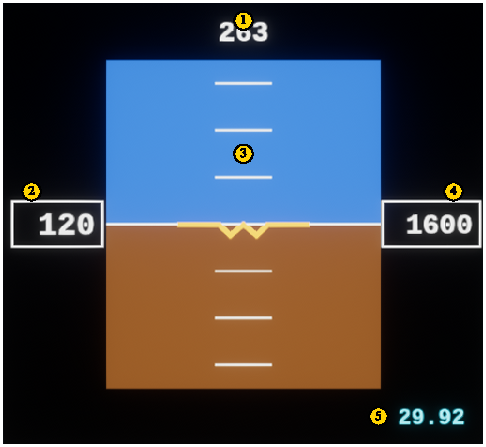
\includegraphics[width=\linewidth]{disp_esfi.pdf}\par\small(a)\end{minipage}\hfill
  \begin{minipage}[c]{0.2\textwidth}\small\begin{enumerate}[label=\textbf{\arabic*},leftmargin=*,itemsep=0pt]
\item heading
\item airspeed
\item attitude
\item altitude
\item altimeter setting
\end{enumerate}
\end{minipage}\hfill
  \begin{minipage}[c]{0.4\textwidth}\centering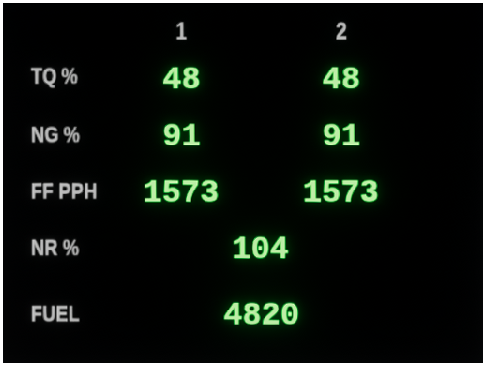
\includegraphics[width=\linewidth]{disp_sfd.pdf}\par\small(b)\end{minipage}
  \caption{The standby instruments: (a) the electronic standby flight instrument, (b) the standby engine and fuel
  display.}\label{fig:esfi}\end{figure}

% =====================================================================================================================
\chapter{Automatic flight control system}\label{ch:afcs}
\section{Description}
The AFCS is a flight director that the augmentation flies when \emph{coupled}. Its modes compute attitudes, the lever
and the nacelles; with CPLD on, the augmentation flies them, and with it off they remain cues. Moving the stick out of
its centre uncouples it (\ann{CPLD OFF}); CPLD couples it again. The coupled AFCS drives the lever while a speed mode is
on: moving the lever flies through it, and left alone for 1.5\,s the AFCS takes it again.

Speed and the flight path share the lever and the pitch as total energy control does: in airplane mode the lever
flies the total energy's rate (climb and acceleration together) and the pitch shares it between climb and speed.
Blended by the nacelle angle from 50 to 80$^\circ$, on the back side of the power curve the lever flies the climb and
the pitch the speed, as a powered-lift aircraft is flown there.

\section{Controls}
The flight control panel's keys and knobs (Table~\ref{tab:panel}), or the keys (Table~\ref{tab:keys}). A hold key takes
the present heading, speed or altitude onto its knob when pressed; the knob then changes it. The knobs' values show in
the panel's windows.
\begin{table}[H]
\centering\small
\caption{The flight control panel.}\label{tab:panel}
\Tab{panel}
\end{table}

\section{Mode annunciation}\label{sec:annunciation}
The mode line along the top of the flight format shows the modes, green when coupled, white as cues: \ann{CPLD}; the
lateral mode (\ann{HDG 270}, \ann{WYPT} and the next waypoint, the approach line's name and \ann{ARM} until it captures);
the vertical (\ann{ALT 2000}, \ann{GP ARM}, \ann{GP 3.0}, \ann{TF 300 MED}); the speed (\ann{SPD 120}); \ann{AUTO NAC};
the approach's phase (\ann{APPR 4.2}, \ann{APPR HOVER}, \ann{APPR LAND}, \ann{APPR DOWN}); the hover hold
(\ann{HVR CPLD DECEL}, \ann{HOLD}, \ann{TRC}, \ann{REM}; \ann{RAD ALT 50}). Alerts show for 5\,s: \ann{CPLD OFF},
\ann{HVR CPLD OFF} (let go), \ann{HVR CPLD UNAVAIL} (refused), \ann{AUTO NAC OFF}, \ann{APPR UNAVAIL},
\ann{VOR/ILS UNAVAIL}, \ann{TF UNAVAIL}.

\section{The modes}
\subsection{Heading hold (HDG HOLD, \key{Ctrl-H})}
Turns to the heading bug (magnetic) and holds it, banking at most 15$^\circ$ at 40\,kt, 20$^\circ$ at 80\,kt and
25$^\circ$ from 150\,kt.

\subsection{Altitude hold (ALT HOLD, \key{Ctrl-A})}
Climbs or descends to the ALT knob's altitude, at up to 1500\,ft/min, and holds it. Engaged in a climb or a descent,
it takes the vertical speed there is and changes it at no more than 0.1\,$g$.

\subsection{Speed hold (SPD HOLD, \key{Ctrl-S})}
Flies the SPEED knob's airspeed, the reference moving to it at 2\,kt/s accelerating and 1.5\,kt/s slowing, and drives
the lever. The reference starts from the aircraft's own airspeed and acceleration and eases into and out of its rate,
at no more than the pitch's 0.1\,$g$ in the exchange of speed for climb (a change of rate of 0.3\,kt/s each second at
120\,kt, 0.15 at 250\,kt), so engaging it slow, or turning the knob, does not pitch the nose. With SPD HOLD on and no
vertical mode it holds the vertical speed it had when engaged.

\subsection{Automatic nacelles (AUTO NAC, \key{U})}
Sets the nacelles for the speed reference from the aircraft's own level-flight trims: at each speed the most converted
angle whose trim pitches the nose up by at most 4$^\circ$ (7$^\circ$ at 180\,kt), within the corridor
(Figure~\ref{fig:corridor}). It needs SPD HOLD (\ann{AUTO NAC (SPD)} without it). Moving the nacelles turns it off
(\ann{AUTO NAC OFF}). With SPD HOLD and AUTO NAC, the SPEED knob alone converts the aircraft either way.

\subsection{Route (WYPT, \key{Ctrl-W})}
Flies the route manager's active route: straight to its first waypoint, then between the legs on its own arcs, started
where an arc at 80\,\% of the bank limit joins them (turns of up to 150$^\circ$). It flies the plan the NAV format draws:
APPR arms with the route, so that from the DECEL point it slows down along the route, descends on the approach path
and comes to a hover over the route's last point; APPR again lands there (Section~\ref{sec:appr}). \ann{WYPT (NO ROUTE)}
shows without an active route.

\subsection{VOR/ILS (\key{Ctrl-N})}
Flies NAV~1's localizer and glide slope, or its VOR on the CRS knob's course, as a line through the station. The line
arms (\ann{ILS 28R ARM}) until the aircraft is within 20\,s of flight of it, the heading or the route flying meanwhile;
with neither on it captures at once. It intercepts at up to 45$^\circ$. The glide path arms (\ann{GP ARM}) and is joined
from below, or from above once past where its descent begins.

\subsection{Approach (APPR, \key{Ctrl-G})}\label{sec:appr}
An approach to a hover 50\,ft over a point, and a landing there:
\begin{itemize}
\item an ILS's threshold, NAV~1 tuned to it;
\item the route's destination runway;
\item the route's last waypoint, a landing zone, approached into the wind at 6$^\circ$.
\end{itemize}
Along the line it slows down at 1.5\,kt/s, as late as it can, and converts with AUTO NAC. Below 35\,kt over the ground
within 2000\,ft of the point it hands over to the hover hold, which holds the hover (\ann{APPR HOVER}). The key again
lands (\ann{APPR LAND}): the height comes down at 2\,ft/s and on the ground the modes go off and the lever comes down
(\ann{APPR DOWN}); pressed before the hover it lands without stopping (\ann{LAND ARM}). A third press turns it off.
Without a line to fly it shows \ann{APPR UNAVAIL}.

\subsection{Go-around (GA, \key{Ctrl-U})}
Ends the approach and the hover hold and flies away: the present heading, the ALT knob's altitude (or 1000\,ft up if
it is not at least 200\,ft above), at the SPEED knob's speed or 80\,kt, with AUTO NAC. \ann{GA} shows until within 100\,ft of
the altitude.

\subsection{Terrain following (TF, \key{Ctrl-T})}
Holds a set clearance over the terrain: the HVR ALT knob's height (200\,ft if it is below 100), or the CDU's \key{T300}
(100--1000\,ft). It engages from 40\,kt over the ground in the air, and turns APPR off; an approach armed later takes
the vertical over from it once its glide path is captured.

It plans a path \MTfHorizon\,s ahead along the track, the lowest that clears the terrain by the clearance, on the track and
150\,ft either side, descending into valleys and pulling up as late as its ride allows, within the climb the engines
can make and 2000\,ft/min of descent. The ride sets its vertical acceleration (\key{R1}, \key{R2}, \key{R3} on the CDU:
soft, medium, hard, 0.1, 0.2 and 0.3\,$g$; medium at the start). It flies the vertical: with SPD HOLD the speed is free
within 20\,kt of the SPEED knob's, so that climbs and descents trade it against height, and held at the band's edges.
The mode line shows \ann{TF 300 MED}.

\DispPair{flt_tf}{the flight format}{nav_tf}{the navigation format, the terrain's profile below}{Terrain following at 300\,ft
over the peninsula's ridge, at 120\,kt.}
Below half the clearance it climbs at full power at 0.5\,$g$ (\ann{FLY UP}); with no terrain data ahead it climbs too
(\ann{TF FAIL}). Pressed again TF ends and the ALT knob takes the present altitude.
\begin{warning}
TF sees terrain \MTfHorizon\,s ahead along the track: enough to climb \MTfRise\,ft at the aircraft's weakest climb,
\MClimbLeast\,ft/min at \MClimbLeastKt\,kt. Higher or nearer terrain, terrain coming into view round a turn, and obstacles the scenery's terrain does not
have can be cleared only as the fly-up allows.
\end{warning}

\subsection{Hover hold (HVR CPLD, \key{y})}
Engaged at up to 40\,kt over the ground with the nacelles past 70$^\circ$, it shows where the aircraft will stop (the
magenta box), stops there at 0.08\,$g$ (\ann{DECEL}) and holds the spot, the heading and the height (\ann{HOLD}):
the radar height below 500\,ft, the barometric above. It moves the lever and the nacelles itself, translating on the
nacelles with the fuselage level.
\begin{itemize}
\item The stick out of its centre flies it over the ground (\ann{TRC}): 10\,kt at half travel, 2\,kt with REM HVR. On
release it stops and holds again.
\item The lever flies through the height hold; left alone for 1.5\,s, the hold takes the new height.
\item Past half the stick's travel, above 45\,kt, below 65$^\circ$ of nacelle or on landing it lets go
(\ann{HVR CPLD OFF}); refused, it shows \ann{HVR CPLD UNAVAIL}.
\end{itemize}

\subsection{Hover height hold (HVR HOLD, \key{Y})}
Holds the HVR ALT knob's radar height, taking the present one when pressed (\ann{RAD ALT 50}).

\section{How the modes combine}
\begin{itemize}
\item \emph{Lateral}: an approach line once captured, else the route (WYPT), else the heading (HDG HOLD). With none the
augmentation holds the bank.
\item \emph{Vertical}: the glide path once captured, else TF, else ALT HOLD, else the vertical speed held by SPD HOLD.
\item \emph{Speed}: SPD HOLD, or the approach's own speed along its path.
\item \emph{The hover hold} takes over all of them while it is on; the approach hands over to it.
\end{itemize}

% =====================================================================================================================
\part{Limitations}
\chapter{Operating limitations}
\section{Conversion corridor}
The nacelle angle shall be kept within the corridor (Figure~\ref{fig:corridor}, Table~\ref{tab:cps}); the conversion
protection holds the command within it.
\begin{figure}[H]
\centering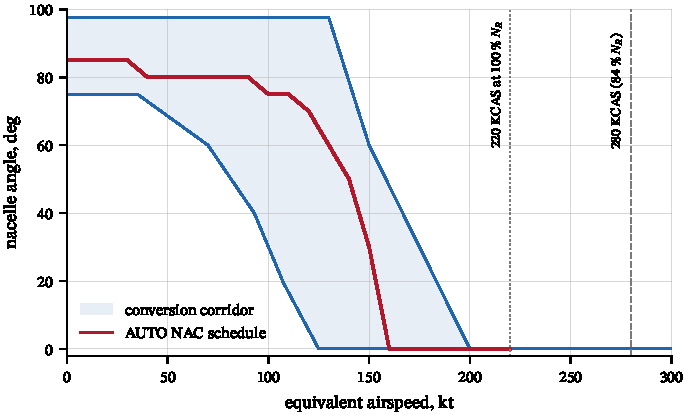
\includegraphics[width=0.8\textwidth]{corridor.pdf}
\caption{The conversion corridor, equivalent airspeed against nacelle angle, with AUTO NAC's schedule and airplane
mode's airspeed limits.}\label{fig:corridor}
\end{figure}
\begin{table}[H]
\centering\small
\caption{The conversion corridor.}\label{tab:cps}
\Tab{cps}
\end{table}

\section{Airspeed}
\begin{itemize}
\item Airplane mode, 84\,\% $N_R$: \MVmo\,KCAS or Mach \MMmo, whichever is less.
\item Airplane mode at 100\,\% $N_R$: \MVmoHundred\,KCAS.
\item Gear down: 150\,KCAS.
\end{itemize}

\section{Rotor speed and power}
\begin{itemize}
\item Rotor speed: \MNrHelo\,\% in helicopter mode and through the conversion, \MNrApln\,\% in airplane mode; \ann{NR}
beyond 3\,\%.
\item Torque: 100\,\% (\ann{TORQUE}). The drive: \MPxmsn\,hp at 100\,\% $N_R$.
\end{itemize}

\section{High sink rate}
\begin{warning}
At low airspeed the rotors can enter their own wake, the vortex ring state, and the aircraft sink fast and roll. The rate of descent shall
stay below \MVrsLoSink\,ft/min up to \MVrsLoKt\,KCAS, rising to \MVrsHiSink\,ft/min at \MVrsHiKt\,KCAS (Figure~\ref{fig:perf}c).
The flight format's vertical speed bar turns amber and red as the descent nears the limit.
\end{warning}

\section{Weight}
\begin{itemize}
\item Maximum vertical take-off: \MWRef\,lb (the reference loading). The hover ceiling (Part~VI) limits it further at
altitude.
\item Cabin load: \MCargoMax\,lb.
\end{itemize}

\section{AFCS}
\begin{itemize}
\item Hover hold: engage below 40\,kt over the ground with the nacelles past 70$^\circ$.
\item TF: from 40\,kt over the ground; clearance 100--1000\,ft.
\item Wing stow: rotors stopped.
\end{itemize}

% =====================================================================================================================
\part{Normal procedures}
\chapter{Normal procedures}
\section{Starting}
On the ground the aircraft starts cold and dark. In the air it starts running and trimmed in level flight at the
start's airspeed, the nacelles at AUTO NAC's angle for it. For the first 5.5\,s it holds still while it trims: the
rotors come up to the aircraft's level-flight trim for the airspeed, its weight, the density altitude and the gear
(down unless raised, FlightGear's default), the nose turns to the trim's pitch, and the collective, the lever and the
stick settle. Then it flies on level, hands off. Slow, heavy and high, past the hover ceiling, the lever is at its
stop and the aircraft sinks.
\begin{enumerate}
\item Thrust control lever: down.
\item AutoStart: \key{\}} (or the V22 Osprey menu). The engines start one after the other; the rotor brake releases.
\item Rotor speed: governed (\MNrHelo\,\%), about 75\,s after the first engine lights.
\end{enumerate}

\section{Vertical take-off and hover}
\begin{enumerate}
\item Nacelles: 90$^\circ$. Gear down.
\item Lever: up smoothly until the aircraft lifts (about two thirds at the start's weight).
\item Hover: hold the attitude with the stick; the heading holds with the pedals centred.
\item To hold the hover: HVR CPLD (\key{y}); HVR HOLD (\key{Y}) holds the radar height.
\end{enumerate}
\begin{note}
The flight format's power bar marks the power to hover in and out of ground effect: with the lever's power past the
out-of-ground-effect mark the aircraft cannot hover clear of the ground.
\end{note}

\section{Conversion to airplane mode}
\begin{enumerate}
\item Accelerate with forward stick, nacelles at 75--80$^\circ$.
\item Nacelles: forward (\key{m}); the protection holds them to the corridor as the speed builds, so the command may be
set fully forward.
\item Gear up above 50\,ft.
\item At 0$^\circ$ the rotor speed comes down to \MNrApln\,\%.
\end{enumerate}
Coupled: SPD HOLD and AUTO NAC, then the SPEED knob to the speed wanted; the AFCS converts at constant altitude with ALT
HOLD.

\section{Airplane mode}
Cruise 240--270\,KCAS. At the slow end of airplane mode the nose is high (\MPitchTwoHundred$^\circ$ at 200\,KCAS against
\MPitchTwoFifty$^\circ$ at 250, Table~\ref{tab:level}): the wing lifts the aircraft alone there.

\section{Conversion to helicopter mode and landing}
\begin{enumerate}
\item Slow down below 200\,KCAS; nacelles up (\key{M}) as the corridor allows; gear down below 150\,KCAS.
\item Approach with the nacelles at 75--85$^\circ$, below the high sink rate limit.
\item Come to a hover over the point, then lower the lever to land.
\item After landing: lever down.
\end{enumerate}

\section{Coupled approach to a hover and landing}
\begin{enumerate}
\item An ILS: NAV~1 tuned to it; or a route whose last point is the landing zone (WYPT).
\item CPLD; HDG HOLD or WYPT, ALT HOLD, SPD HOLD, AUTO NAC.
\item APPR (\key{Ctrl-G}): the line arms and is drawn on the NAV format; it captures within 20\,s of flight of it.
\item The AFCS descends on the path, slows down and hands over to the hover hold 50\,ft over the point.
\item APPR again: it lands, and the lever comes down on the ground.
\end{enumerate}
With a route flown by WYPT, APPR arms itself.

\section{Terrain following}
\begin{enumerate}
\item CPLD; HDG HOLD or WYPT; SPD HOLD, AUTO NAC.
\item Clearance: the HVR ALT knob, or \key{T300} on the CDU. Ride: \key{R1}--\key{R3}.
\item TF (\key{Ctrl-T}). Check \ann{TF 300 MED} on the mode line.
\item To end it: TF again; the ALT knob takes the present altitude, and ALT HOLD holds it.
\end{enumerate}

\section{Shutdown}
\begin{enumerate}
\item Lever down; AutoStop: \key{\}}.
\item To stow: wing (\key{N}) once the rotors have stopped.
\end{enumerate}

% =====================================================================================================================
\part{Flight characteristics}
\chapter{Flight characteristics}
\section{Hover and low speed}
With attitude command the aircraft holds the attitude the stick sets, so it stays where it is put; the drift is
flown with small attitude changes. In ground effect it needs less power: the power bar shows both. Descending slowly
at low speed, mind the high sink rate boundary.

\section{The conversion}
Hands off, the trim schedule holds the attitude through the conversion; the nacelles move at up to
\MNacRate$^\circ$/s. Converting, the aircraft accelerates on the nacelles' tilt rather than on its pitch; the pitch
attitude changes a few degrees at each angle (Table~\ref{tab:level}).

\section{Airplane mode}
The wing carries the aircraft above about 180\,KCAS; at its slow end the nose is \MPitchTwoHundred$^\circ$ up, at cruise
\MPitchTwoSeventy--\MPitchTwoFifty$^\circ$.
\begin{table}[H]
\centering\small
\caption{Level flight along AUTO NAC's schedule at \MWRef\,lb, 1000\,ft: the power required, the pitch attitude, and
whether one engine (\MPoneThousand\,hp there) holds it.}\label{tab:level}
\Tab{level}
\end{table}

\section{Under the AFCS}
Coupled, the AFCS flies the augmentation's attitudes and their rates, the stick for those rates fed forward from the
aircraft's own response, so it turns and pulls up without lag or overshoot. In TF the climbs and descents trade the
speed within its band; over hills higher than the ride lets it follow at high speed it stays above the valleys.

% =====================================================================================================================
\part{Emergency procedures}
\chapter{Emergency procedures}
\section{Engine failure}
\ann{ENG 1 OUT} or \ann{ENG 2 OUT}. The interconnect shaft drives both rotors from the remaining engine, which gives
up to its own rating, \MPmrp\,shp at sea level, against the \MPxmsn\,hp the drive passes with both. At the reference
loading one engine holds level flight from \MOeiLo\,KCAS in the conversion and in airplane mode up to 250\,KCAS, not
in the hover (\MOeiHoverPower\,hp at 40\,kt) nor at 120--160\,KCAS (Table~\ref{tab:level}).
\begin{enumerate}
\item In the hover or at low speed: land, or accelerate to 80--100\,KCAS with the nacelles at 75--80$^\circ$ if clear of
the ground.
\item In the conversion: continue to airplane mode, or back to 80--100\,KCAS.
\item In airplane mode: 180--250\,KCAS; land as soon as practicable, converting as the speed allows.
\end{enumerate}
\begin{warning}
Below 80\,KCAS and at 120--160\,KCAS, at the reference loading, one engine cannot hold level flight.
\end{warning}

\section{High sink rate}
Nacelles forward and the nose down to gain airspeed; do not pull the lever up alone, which deepens the vortex ring state.

\section{Conversion protection}
\ann{CONV PROT}: the nacelles held off the command by the corridor. Fly the speed into the corridor for the angle
commanded, or bring the command to the nacelles.

\section{AFCS}
\begin{itemize}
\item \ann{CPLD OFF}: uncoupled by the stick. Fly the aircraft; CPLD to couple again.
\item \ann{HVR CPLD OFF}: the hover hold let go. Fly the hover; HVR CPLD again once within its limits.
\item \ann{FLY UP}: TF below half its clearance, climbing at full power. Let it climb; if it persists, climb to a safe
altitude and end TF.
\item \ann{TF FAIL}: no terrain data ahead; TF climbs. End TF and fly at a safe altitude.
\end{itemize}

% =====================================================================================================================
\part{Performance data}
\chapter{Performance}
The flight model's own; its report compares it with the published data.
\begin{figure}[H]
\centering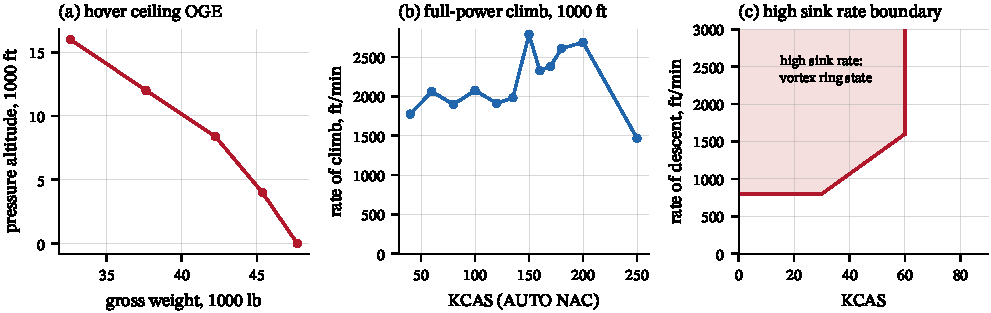
\includegraphics[width=\textwidth]{perf.pdf}
\caption{(a) The hover ceiling out of ground effect, standard day, 100\,\% $N_R$; (b) the climb at full power along
AUTO NAC's schedule at \MClimbWeight\,lb, 1000\,ft; (c) the high sink rate boundary.}\label{fig:perf}
\end{figure}
\begin{table}[H]
\centering\small
\begin{minipage}{0.45\textwidth}\centering
\caption{Hover ceiling OGE, standard day.}
\Tab{ceiling}
\end{minipage}\hfill
\begin{minipage}{0.5\textwidth}\centering
\caption{Maximum level speed, airplane mode.}
\Tab{vmax}
\end{minipage}
\end{table}

% =====================================================================================================================
\appendix
\chapter{Keys}
\begin{table}[H]
\centering\small
\caption{Keys.}\label{tab:keys}
\Tab{keys}
\end{table}

\end{document}
